%% LyX 2.3.2-2 created this file.  For more info, see http://www.lyx.org/.
%% Do not edit unless you really know what you are doing.
\documentclass[oneside,english]{amsart}
\usepackage[T1]{fontenc}
\usepackage[latin9]{inputenc}
\usepackage{amsthm}
\usepackage[authoryear]{natbib}
\usepackage{endnotes}
\usepackage{graphicx}
\usepackage{url}

\makeatletter
%%%%%%%%%%%%%%%%%%%%%%%%%%%%%% Textclass specific LaTeX commands.
\numberwithin{equation}{section}
\numberwithin{figure}{section}
\theoremstyle{plain}
\newtheorem{thm}{\protect\theoremname}
\theoremstyle{definition}
\newtheorem{defn}[thm]{\protect\definitionname}

\makeatother

\usepackage{babel}
\providecommand{\definitionname}{Definition}
\providecommand{\theoremname}{Theorem}

\begin{document}

\section{Euclidean hyperspherical embedding of networks}

In this work we consider undirected connected simple graphs $\Gamma=\left(V,E\right)$,
where $V$ is the set of vertices or nodes and $E$is the set of edges.
Let $A=A\left(\Gamma\right)=\left[A_{ij}\right]_{n\times n}$ be the
adjacency matrix of $\Gamma$. Because the graphs considered here
are undirected the associated adjacency matrix is symmetric, and its
eigenvalues are real. We label the eigenvalues of $A$ in non-increasing
order: $\lambda_{1}>\lambda_{2}\geq\ldots\geq\lambda_{n}$. Since
$A$ is a real-valued, symmetric matrix, we can decompose $A$ into
$A=U\Lambda U^{T}$, where $\Lambda$ is a diagonal matrix containing
the eigenvalues of $A$ and $U=[\mathbf{\overrightarrow{\psi}}_{1},\ldots,\mathbf{\overrightarrow{\psi}}_{n}]$
is orthogonal, where $\mathbf{\overrightarrow{\psi}}_{i}$ is an eigenvector
associated with $\lambda_{i}$. We denote by $\mathbf{\mathbf{\psi}}_{j,u}$
the $u$th entry of the $j$ th eigenvector of $A$. A row of the
matrix $U$ corresponding to the node $i$ of the graph is designated
here by the vector $\vec{\varphi}_{i}=\left[\mathbf{\mathbf{\psi}}_{1,i},\ldots\mathbf{\mathbf{\psi}}_{n,i}\right]^{T}$.

An important quantity for studying communication processes in networks
is the so-called communicability function \citet{Communicability,Estrada_Higham,Estrada_Hatano_Benzi},
which is defined as follows.
\begin{defn}
Let $u$ and $v$ be two nodes of $\Gamma$, then the communicability
function between these two nodes is

\begin{equation}
G_{uv}=\sum_{k=0}^{\infty}\frac{\left(A^{k}\right)_{uv}}{k!}=\left(\exp\left(A\right)\right)_{uv}=\sum_{k=1}^{n}e^{\lambda_{k}}\mathbf{\mathbf{\psi}}_{k,u}\mathbf{\psi}_{k,v}.
\end{equation}
\end{defn}

It counts the total number of walks starting at node $u$ and ending
at node $v$, weighted in decreasing order of their length by a factor
$\frac{1}{k!}$. That is, the communicability function considers shorter
walks more influential than longer ones and penalize them appropriately
such that the whole series converges. The $G_{uu}$ terms of the communicability
function characterize the degree of participation of a node in all
subgraphs of the network, giving more weight to the smaller ones.
Thus, it is known as the subgraph centrality of the corresponding
node \citet{Subgraph_Centrality}.

Let us now define a parameter that account for the difference between
the number of weighted closed walks that start at (and return to)
the corresponding nodes $u$ and $v$, and the number of weighted
walks that start at node $u$ (respectively $v)$ and ends at the
node $v$ (respectively $u).$
\begin{defn}
Let $u$ and $v$ be two nodes of $\Gamma$, then
\end{defn}

\begin{equation}
\xi_{uv}^{2}=G_{uu}+G_{vv}-2G_{uv}
\end{equation}

This difference, which is defined below as $\xi_{uv}^{2}$ serves
as a quantification of the potential quality of communication channels
between two nodes. That is, if there are many routes that connect
nodes $u$ and $v$ together, and there are not many routes that starting
at the node $u$ (respectively $v)$ return to it, we can say that
most of ``information'' departing the node $u$ (respectively $v)$
with destination to the node $v$ (respectively $u)$ will arrive
at it. Thus, there is a potential good quality of communication between
these two nodes. The other way around is very clear as if there are
many returning routes to the nodes and very few connecting them, most
of the information departing one node will hardly arrive at the other.
In a similar way we can define the ratio between the communicability
between the two nodes and the product of the self-communicabilities
of both nodes.
\begin{defn}
Let $u$ and $v$ be two nodes of $\Gamma$, then
\end{defn}

\begin{equation}
\gamma_{uv}=\dfrac{G_{uv}}{\sqrt{G_{uu}G_{vv}}}.\label{eq:comm_angle}
\end{equation}

Then, we have proved the following result.
\begin{thm}
Let $u$ and $v$ be two nodes of $\Gamma$, and let $\xi_{uv}^{2}$
and $\gamma_{uv}$ the parameters defined before. Then, $\xi_{uv}^{2}$
is a square Euclidean distance between the two nodes and $\theta_{uv}=\cos^{-1}\gamma_{uv}$
is the Euclidean angle spanned between the positions vectors of the
two nodes in a Euclidean space.
\end{thm}

Althought we are not proving the result here we sketch the procedure
of its proof. The matrix $G=\exp\left(A\right)$ is positive define,
and so we can express it as a Gram matrix of the form

\begin{equation}
G=X^{T}X,
\end{equation}
where $X=\left[\vec{x}_{1},\ldots,\vec{x}_{n}\right]$ and

\begin{equation}
\vec{x}_{u}=\exp\left(\varLambda/2\right)\vec{\varphi}_{u},
\end{equation}

Then, it is straightforward to realize that

\begin{equation}
\begin{array}{lll}
\vec{x}_{u}\cdot\vec{x}_{u} & =\left(\exp\left(\varLambda/2\right)\vec{\varphi}_{u}\right)^{T}\exp\left(\varLambda/2\right)\vec{\varphi}_{v}\\
 & =\vec{\varphi}_{u}^{T}\exp\left(\varLambda/2\right)\exp\left(\varLambda/2\right)\vec{\varphi}_{v}\\
 & =\vec{\varphi}_{u}^{T}\exp\left(\varLambda\right)\vec{\varphi}_{v}\\
 & =\sum_{k=1}^{n}e^{\lambda_{k}}\mathbf{\mathbf{\psi}}_{k,u}\mathbf{\psi}_{k,v}\\
 & =G_{uv.}
\end{array}
\end{equation}
Then, we can express $\xi_{uv}^{2}$ in terms of the vectors $\vec{x}_{u}$
and $\vec{x}_{v}$ as 
\begin{equation}
\begin{array}{ll}
\xi_{uv}^{2} & =\vec{x}_{u}\cdot\vec{x}_{u}+\vec{x}_{v}\cdot\vec{x}_{v}-2\vec{x}_{u}\cdot\vec{x}_{v}\\
 & =\left\Vert \vec{x}_{u}-\vec{x}_{v}\right\Vert ^{2},
\end{array}
\end{equation}
which means that $\xi_{uv}^{2}$ is a Euclidean distance (metric)
between the corresponding nodes and that $\vec{x}_{u}$ is the position
vector of the corresponding node in such Euclidean space. It is now
obvious that

\begin{equation}
\cos\theta_{uv}=\dfrac{\vec{x}_{u}\cdot\vec{x}_{v}}{\left\Vert \vec{x}_{u}\right\Vert \left\Vert \vec{x}_{v}\right\Vert }=\dfrac{G_{uv}}{\sqrt{G_{uu}G_{vv}}}=\gamma_{uv}.
\end{equation}

It is important to remark here that the embedding induced by the communicability
function is in a Euclidean hypersphere as proved in the following
result.
\begin{thm}
Let $\Gamma$ be a simple connected graph. Then, $\vec{x}_{u}$ is
a vector pointing from the origin of an $\left(n-1\right)$-sphere
to its surface where the node $u$ is located. The radius of this
hypersphere is given by \citet{Angles}

\begin{equation}
R^{2}=\frac{1}{4}\left(c-\frac{\left(2-b\right)^{2}}{a}\right),
\end{equation}
where $a=\vec{1}^{T}\exp\left(-A\right)\vec{1}$, $b=\vec{s}^{T}\exp\left(-A\right)\vec{1}$,
$c=\vec{s}^{T}\exp\left(-A\right)\vec{s}$, and $\vec{s}={\rm diag}(\exp\left(A\right))$.
\end{thm}

This means that the communicability function induces an embedding
of every connected simple graph of $n$ nodes into the surface of
a Euclidean $\left(n-1\right)$-sphere. The case of two graphs with
3 nodes is illustrated in Fig. XX.

\section{The problem of visualization}
We implemented the framework described in the previous section using scientific,
database and web resources, making it available within a web page\endnote{Available at: \url{http://rfabbri.vicg.icmc.usp.br:3000/communicability}.}
for use through simple mouse-driven actions and requiring no software installation beyond a web browser. % such as Firefox or Google Chrome.
The software has been named ComNetVis (from Communicability-based Network Visualization)
and is exemplified in Figures~\ref{fpage0},~\ref{finitial},~\ref{fcom},~\ref{flay}, and~\ref{fsecond}.
In this section we describe its functionalities and the underlying technologies.

\begin{figure*}\centering
 \includegraphics[width=\textwidth]{figs/overall}
  \caption{The ComNetVis interface: 
  (1) drop-down menu for selecting or uploading a network for analysis;
  (2) widgets for setting the communicability calculations;
  (3) widgets for setting the community detection;
  (4) widgets for setting the node-link layout;
  (5) the render button to display the network;
  (6) toolbar with controls for fine-tuning the visualization and downloading the image and communities;
  (7) interactive table holding information about the communities;
  can also be used to set the visualization on the canvas;
  (8) canvas with the node-link representation of the network.
  (9) text areas for further information about the visualization achieved.
  Notice that nodes shown belong to six communities, each with the color and size denoted in the table (7).
  These elements are further described in this section.
  }\label{fpage0}
\end{figure*}

In using ComNetVis, the analyst first uses a drop-down menu to select
a network of interest, s/he may also upload a new network using the same menu.
Then s/he sets parameters for the calculation of the communicability angles, as illustrated in Figure~\ref{finitial}, although default settings are reasonable, specially for a newcomer.
The next step is to set the community detection algorithm.
To do so, the user selects a dimensionality reduction method, and a target dimensionality in which clustering is going to be performed.
Accordingly, s/he selects a clustering algorithm and the minimum and maximum number of communities of interest, as illustrated in Figure~\ref{fcom}.
The last step, before the achievement of the visual mapping,
is to set the node-link layout algorithm:
the user selects a dimensionality reduction method,
and the number of dimensions of the layout,
as illustrated in Figure~\ref{flay}.

Theoretically,
any dimensionality reduction method
and any clustering algorithm
can be used.
In this interface, to encompass a reasonable collection of techniques,
and enable the proof-of-concept,
we implemented five dimensionality reduction methods
(PCA~\cite{pca}, t-SNE~\cite{tsne}, Locally Linear Embedding~\cite{lle},
ISOMAP~\cite{isomap}, and MDS~\cite{mds}),
and three clustering algorithms (k-means,
Ward's hierarchical~\cite{ward}, and spectral~\cite{spectral}).



\begin{figure}\centering
 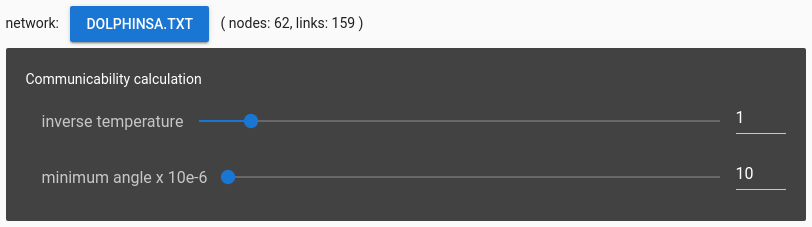
\includegraphics[width=\columnwidth]{figs/initial}
  \caption{The initial step of the ComNetVis usage is to apply the communicability calculation to an input network.
  The button at the top is for network uploading and selection.
  In the gray box the user chooses the inverse temperature and the minimum angle.
  }\label{finitial}
\end{figure}


\begin{figure}\centering
 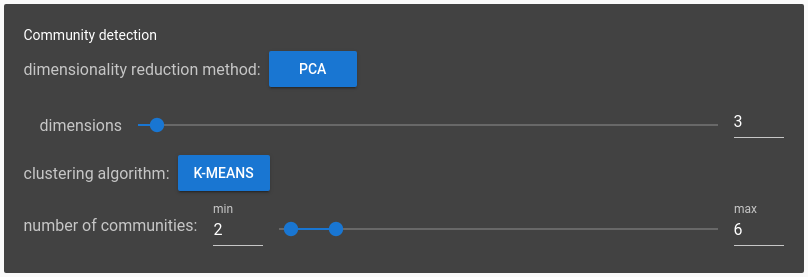
\includegraphics[width=\columnwidth]{figs/com}
  \caption{
    Settings of the community detection: the dimensionality reduction method;
    the target dimensionality in which the communities are going to be found;
    the clustering algorithm;
    and the minimum and maximum number of communities.
  }\label{fcom}
\end{figure}

\begin{figure}\centering
 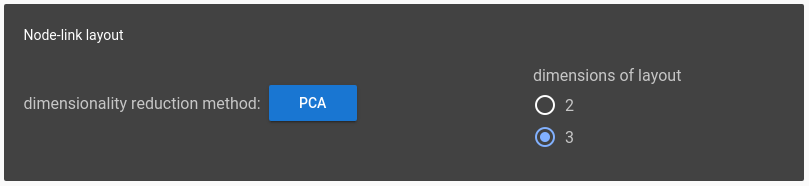
\includegraphics[width=\columnwidth]{figs/lay}
  \caption{
    Settings of the layout: the dimensionality reduction method and
    the number of dimensions of the layout, which can be 2 or 3.
  }\label{flay}
\end{figure}

Once the ``render network'' button is hit,
the network node-link representation is mapped to the screen
according to the selected settings.
Subsequent usage relies on manipulation of the visual mapping, using control elements presented with the canvas, by means of mouse operations.
These procedures are illustrated in Figure~\ref{fsecond}:
changing overall node size or proportionality to degree;
changing node and link transparency;
visualization of the centroid and best sphere center and surface;
download of image and of communities;
changing the colors and the number of communities.

\begin{figure*}\centering
 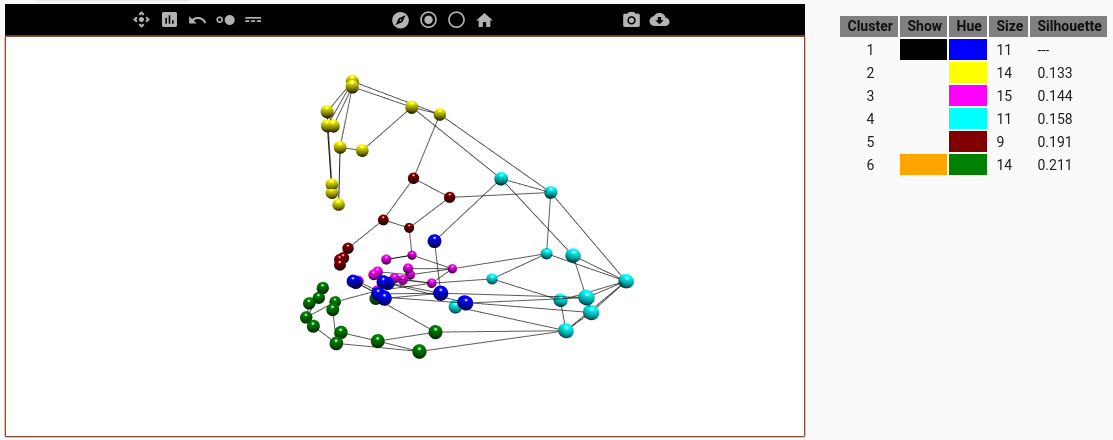
\includegraphics[width=\textwidth]{figs/second}
  \caption{
    Second phase of ComNetVis usage which takes place with the network mapped to the canvas.
    The network can be rotated or translated by click and drag or Ctrl-click and drag, respectively, in the canvas.
    The toolbar, above the canvas, holds three sets of buttons.
    The first set of buttons, at the left, enables:
    increase/decrease of node size;
    emphasize node size proportionality to degree;
    reset node proportionality;
    increase/decrease node transparency; and
    increase/decrease link transparency.
    The middle set of buttons enables:
    show/hide centroid;
    show/hide best sphere center;
    show/hide best sphere surface; and
    recover initial position.
    The last set of buttons enables:
    save image; and
    download communities as a CSV file.
    The table, to the right, allows the analyst to change the number of communities associated to the network, and to change the color of the community, by
    clicking on the columns ``Show'' and ``Hue'', respectively.
    The ``Size'' of each community changes in the table when the user changes the number of communities.
    The ``Silhouette'' score is a measure of how consistent are the clusters:
    higher values are associated to better clusters.
  }\label{fsecond}
\end{figure*}

\subsubsection{Underlying software technologies:}
% coarsening algorithms
% flask for server, feather for auxiliary server
% mongodb filesystem for data
% Nuxt/Vue.js for the frontend with heavy use of PIXI.js
Components of ComNetVis are written in a combination of JavaScript and Python: Vue.js (set up by Nuxt.js) is used for the front-end client, the back-end is a Flask Python server, used to perform specialized or heavy calculations.
A secondary server, a FeatherJS, is used to facilitate database-related operations and real-time multi-user interaction.
The data is stored in a MongoDB database,
while the multi-user interaction is deactivated for now to avoid unnecessary complexity.
The communicability-related calculations for community detection and network layout are performed by the Flask server.
The fast WebGL 3D rendering on the canvas is performed using Babylon.js.

\subsection{Use cases}

\section{Conclusions and further work}
\subsection*{Acknowledgement}
The authors acknowledge the financial support of the S\~ao Paulo State Research Foundation (FAPESP grant 2017/05838-3).
The views expressed do not reflect the official policy or position of FAPESP or CNPq.

\appendix
\section{Ranking of the algorithms by computational cost}
The dimensionality reduction methods, listed from 
slowest to fastest, are:
MDS,
Isomap,
Locally Linear Embedding,
t-SNE,
and PCA.
By far, PCA is the fastest of these methods\endnote{As described in~\url{https://umap-learn.readthedocs.io/en/latest/benchmarking.html}.}.

% put UMAP on the methods again?

The clustering methods, 
listed from the one that scales worst to best:
spectral,
Ward's hierarchical,
k-means\endnote{As described in~\url{https://scikit-learn.org/stable/modules/clustering.html\#clustering}.}.

\theendnotes
\bibliographystyle{plain}
\bibliography{mbib}

\end{document}
